\section{Specification and Design}
\label{sec:design}

\begin{guidance}[Specification and design (15 marks)]
Required (brief, A.3--A.5): an \textbf{embedded server FSM} covering IDLE,
IN\_PROGRESS, GAME\_OVER \textbf{and the move-validation branch}; a
\textbf{flowchart of the GUI application}; and a \textbf{circuit diagram} of the
STM-to-PC UART connection, with the on-board button and LED behaviour labelled.
Diagrams may be at function level. Explain \textbf{why} responsibilities sit on
the server or the client. Draw diagrams in a tool that exports vector PDF
(draw.io, TikZ, Mermaid) and check that every label is readable when printed.
\end{guidance}

\subsection{System Architecture and Separation of Concerns}
The system enforces a clean client-server divide designed around a zero-trust model: the PC client is treated as an untrusted rendering terminal, while the STM32F051 microcontroller functions as the authoritative arbiter. Table~\ref{tab:responsibilities} summarizes the allocation of responsibilities between the two domains.

The embedded firmware is decoupled into four modular subsystems:
\begin{enumerate}
    \item \textbf{Protocol Framing (\texttt{protocol.c})}: Ingests raw UART bytes via interrupt, validates frame boundaries and character sets, enforces inter-byte timeouts, and formats outbound ASCII packets.
    \item \textbf{Game Logic and FSM (\texttt{battleship.c})}: Maintains the single source of truth for grid state, evaluates move validity, coordinates atomic fleet placement, tracks fleet damage, and dictates state transitions.
    \item \textbf{Peripheral Hardware (\texttt{hardware.c})}: Manages low-level GPIO operations, button debouncing, LED health bar representation, and turn indicators.
    \item \textbf{Probability Heatmap AI (\texttt{ai.c})}: Generates legal fleet placements and autonomous targeting coordinates directly on the Cortex-M0.
\end{enumerate}

Conversely, the PC application is strictly decoupled from game rules. The GUI captures raw mouse clicks, translates them into coordinate strings, and transmits them over UART. The client cannot locally mark a cell as hit, miss, or sunken, nor can it advance turns. All interface mutations occur solely in response to authoritative microcontroller confirmations.

\begin{table}[t]
\centering
\caption{Allocation of responsibilities between PC and STM32.}
\label{tab:responsibilities}
\footnotesize
\begin{tabular}{@{}L{2.4cm}L{2.7cm}L{2.9cm}@{}}
\toprule
Domain & STM32 Server & PC GUI Client \\
\midrule
Fleet Layouts & Authoritative storage in internal SRAM (secret). & Local cache populated strictly upon server confirmation. \\
Turn Tracking & Authoritative counter (\texttt{current\_turn}). & Reflects server-directed turn state; locks inputs out-of-turn. \\
Move Legality & Validates syntax, bounds, turn, and prior hits. & Forwards raw click; cannot evaluate legality. \\
Hit / Miss / Win & Computes cell intersection and damage. & Renders sprites according to received server token. \\
Hardware I/O & GPIO LEDs, debounced push-button, USART. & Virtual COM Port communication via background thread. \\
\bottomrule
\end{tabular}
\end{table}

\begin{figure*}[t]
\centering
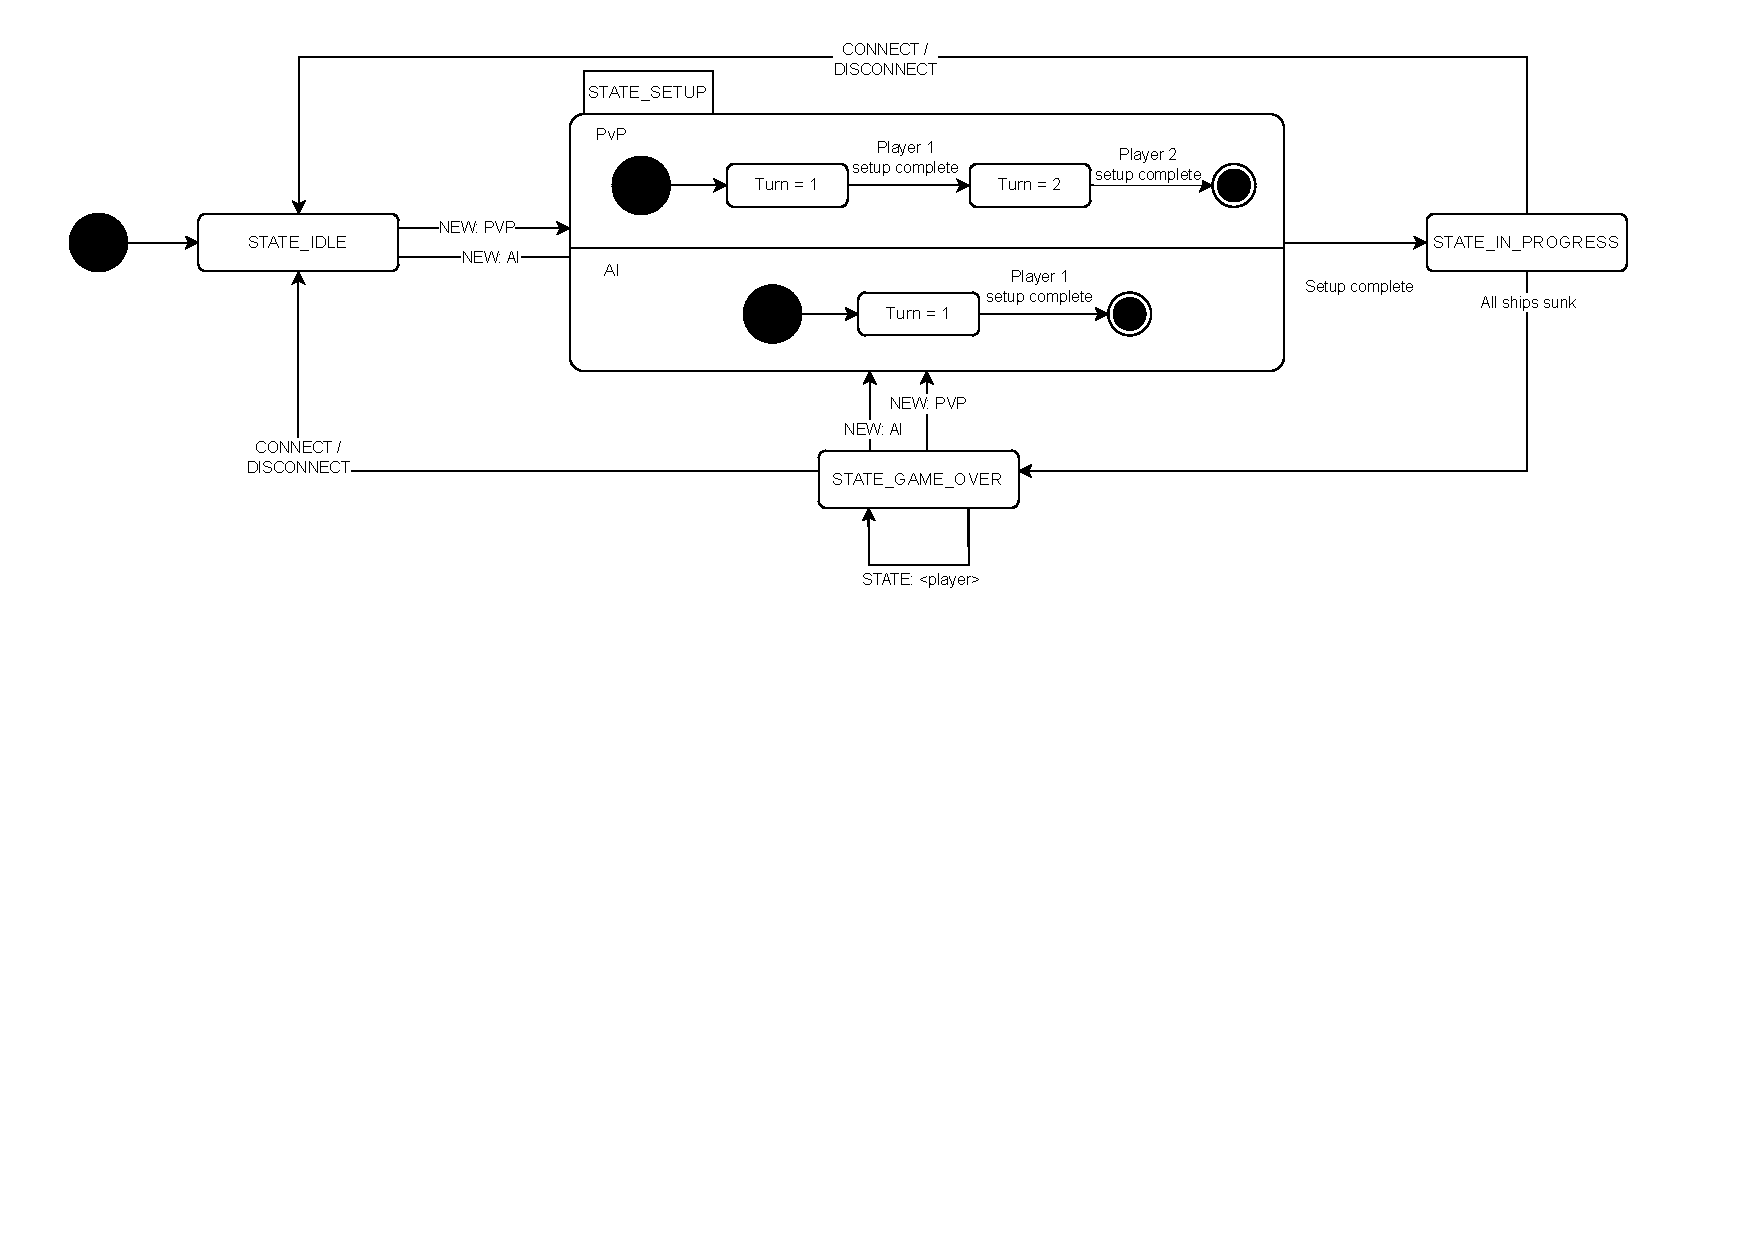
\includegraphics[width=0.82\textwidth]{figures/FSM_diagram.pdf}
\caption{Embedded server finite-state machine (FSM) showing top-level state transitions and the move-validation branch. Any failed check exits immediately with a specific NACK, leaving the grid state completely unmodified.}
\label{fig:fsm}
\end{figure*}

\subsection{Embedded Server Finite-State Machine}
The embedded server FSM (Fig.~\ref{fig:fsm}) implements four operational states and a deterministic validation tree:
\begin{itemize}
    \item \textbf{\texttt{STATE\_IDLE}}: Bootstrapping state. Configures clocks, peripherals, and interrupt lines. Ignores combat actions with \texttt{NACK: NOGAME}. Acknowledges \texttt{CONNECT} and initializes session variables. Transition to \texttt{STATE\_SETUP} occurs upon receiving \texttt{NEW: PVP} or \texttt{NEW: AI}.
    \item \textbf{\texttt{STATE\_SETUP}}: Enforces atomic fleet positioning via \texttt{FLEET: <p>,<coords...>}. In Player-vs-Player (PVP) mode, Player~1 placement yields \texttt{OK: SETUP\_P2} and advances \texttt{current\_turn = 2}; Player~2 placement completes setup and advances to \texttt{STATE\_IN\_PROGRESS}. In AI mode, Player~1 placement immediately triggers on-board AI fleet generation, initializes the AI hunt/target engine, and transitions directly to combat.
    \item \textbf{\texttt{STATE\_IN\_PROGRESS}}: Active gameplay loop. As illustrated in Fig.~\ref{fig:fsm}, every incoming \texttt{SHOOT} command passes through a sequential validation pipeline:
    \begin{enumerate}
        \item \textit{Turn Lock}: Ensures the acting player corresponds to \texttt{current\_turn}, guarding against out-of-order execution (\texttt{NACK: NOTURN}).
        \item \textit{Coordinate Range}: Validates that row and column indices reside strictly within $[0, 9]$ (\texttt{NACK: BADCOORDS}).
        \item \textit{Duplicate Shot}: Inspects bit $0\text{x}80$ of the target cell. If already set, rejects duplicate firing without consuming the player's turn (\texttt{NACK: REPEAT}).
        \item \textit{Damage Evaluation}: Marks the cell with bit $0\text{x}80$. If the cell contains \texttt{SHIP\_NONE}, emits \texttt{MISS} and toggles turns. If a vessel is present, increments damage counters, emitting \texttt{HIT} or \texttt{SUNK}.
        \item \textit{Terminal Condition}: Sinking the 5th fleet vessel satisfies the win predicate, broadcasting \texttt{WIN} and entering \texttt{STATE\_GAME\_OVER}.
    \end{enumerate}
    \item \textbf{\texttt{STATE\_GAME\_OVER}}: Combat is permanently halted. Any subsequent shot yields \texttt{NACK: OUT\_OF\_STATE,GAME\_OVER}. Status LEDs alternate in a 250\,ms blinking pattern. Responds to \texttt{STATE: 2} by returning the full AI fleet to populate the end-game review screen, or accepts \texttt{NEW} to commence a new match.
\end{itemize}

\begin{figure}[t]
\centering
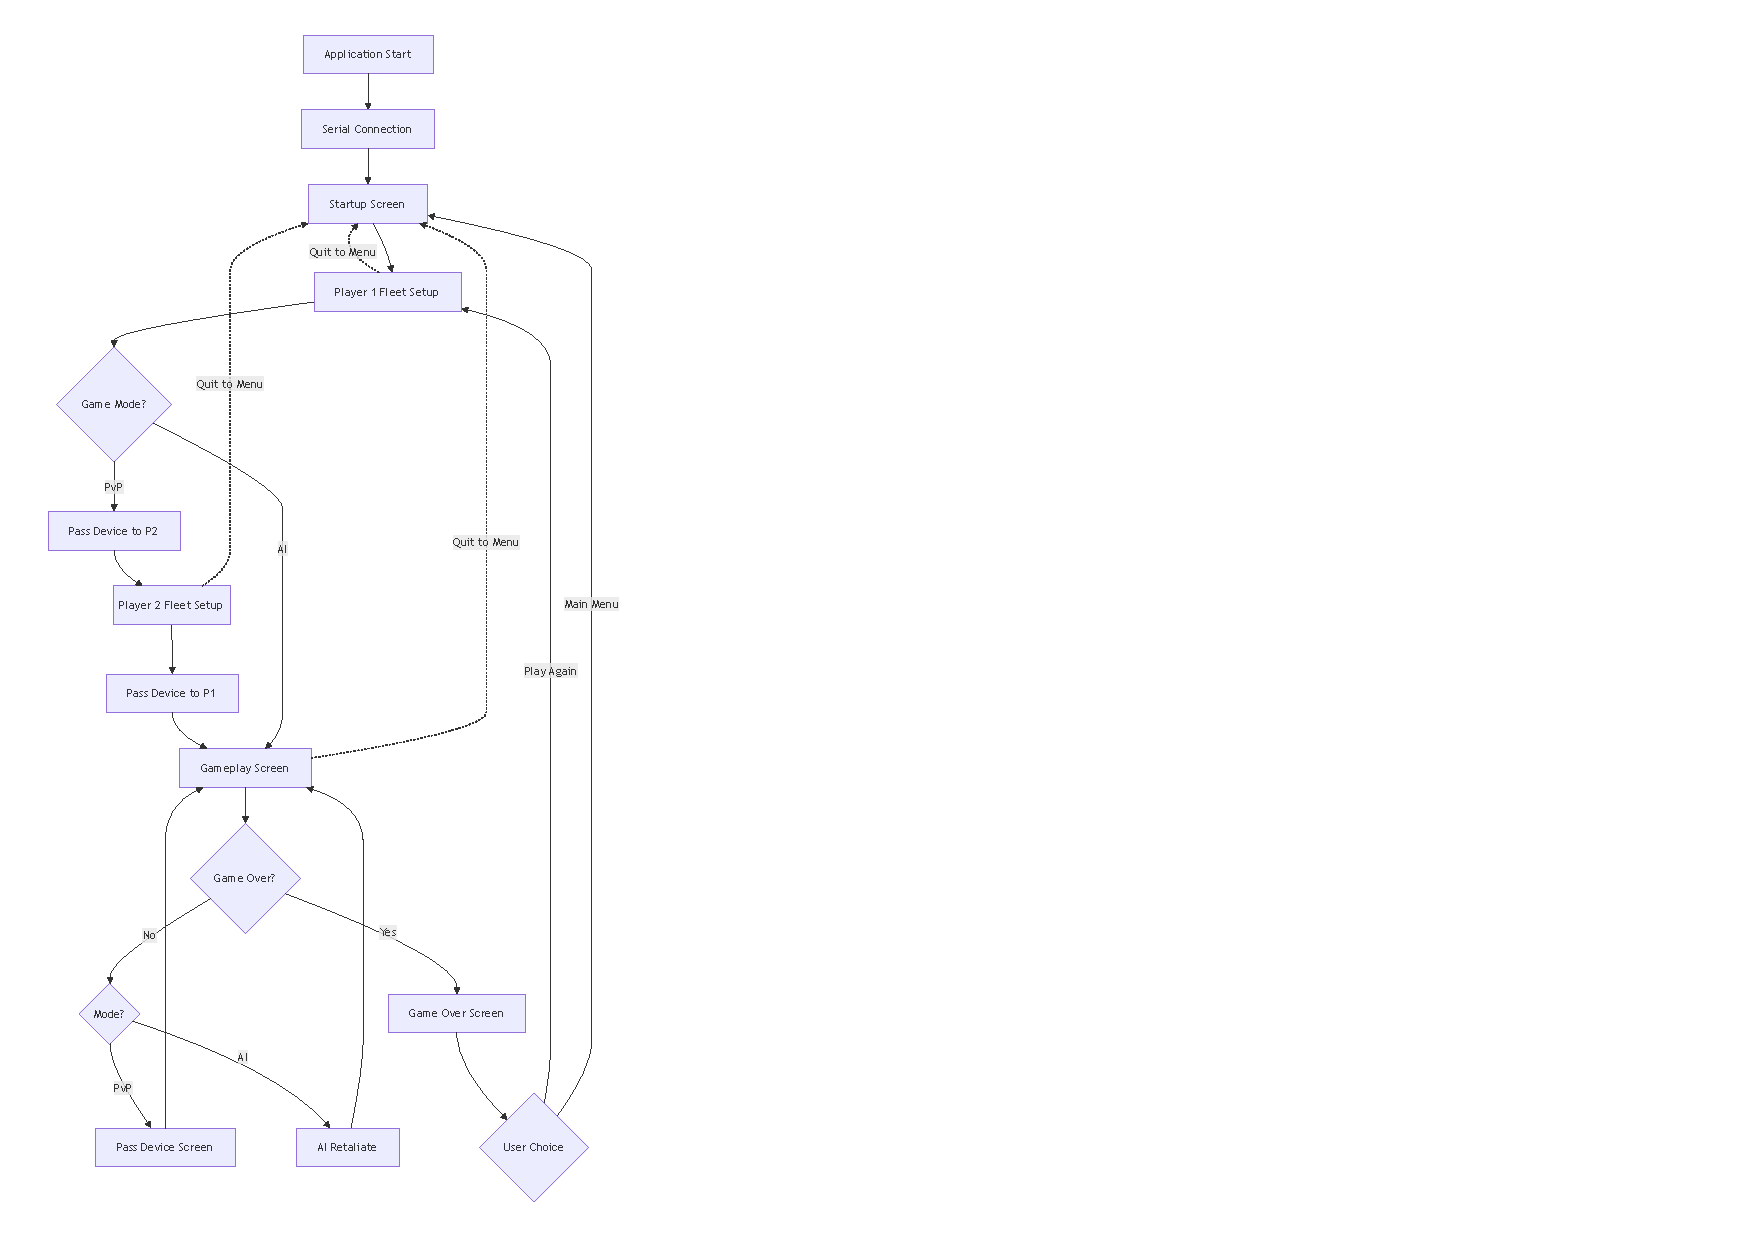
\includegraphics[width=0.88\columnwidth]{figures/GUI_diagram.pdf}
\caption{PC GUI client application flowchart illustrating connection discovery, fleet deployment pathways, turn sequencing, and game-over resolution.}
\label{fig:gui}
\end{figure}

\subsection{PC GUI Client Flowchart and Concurrency Architecture}
The PC client application architecture (Fig.~\ref{fig:gui}) is structured as a finite stack of views managed by a central \texttt{QStackedWidget} in \texttt{MainWindow}:
\begin{enumerate}
    \item \textbf{Startup and Auto-Discovery}: On launch, \texttt{SerialWorker} queries all system COM ports. It scans hardware description strings for ST-LINK and standard USB-to-UART bridge signatures, connecting automatically without requiring manual port entry.
    \item \textbf{Fleet Setup and Masking}: Players position ships using visual snap-to-grid controls. In PVP mode, to prevent screen-peeking during local hotseat play, the application inserts a \texttt{PassDeviceScreen} between Player~1 and Player~2 setup phases, ensuring fleet layouts remain concealed.
    \item \textbf{Gameplay Loop}: During active play, the GUI renders two separate grids: the active player's secret \textit{Home Fleet} (showing ships and incoming enemy fire) and the \textit{Target Radar} (displaying confirmed shots). Clicking a radar cell immediately locks the UI, transmits the \texttt{SHOOT} command, and awaits microcontroller resolution.
    \item \textbf{Game Over and Fleet Reveal}: Upon receiving \texttt{WIN}, the client queries the server for the opponent's true coordinates (\texttt{STATE: 2}), transitioning to the \texttt{GameOverScreen} where sunken vessels and unhit enemy ships are fully revealed.
\end{enumerate}

To ensure complete responsiveness, all serial communications are executed asynchronously within a dedicated \texttt{QThread} subclass (\texttt{SerialWorker}). Communication between the worker thread and the GUI relies exclusively on thread-safe Qt signals and slots:
\begin{itemize}
    \item Outbound frames are placed into a thread-safe FIFO queue (\texttt{queue.Queue}) via the slot \texttt{send\_command()}, where the background thread drains and transmits bytes over UART.
    \item Inbound lines are read non-blockingly via \texttt{readline()}, stripped of delimiters, and emitted through the \texttt{message\_received(str)} signal directly into the main thread router \texttt{handle\_server\_response()}.
\end{itemize}
This threading design guarantees that serial transmission latencies or hardware timeouts never block the main Qt event loop, preventing UI freezing or frame dropping.

\begin{figure}[t]
\centering
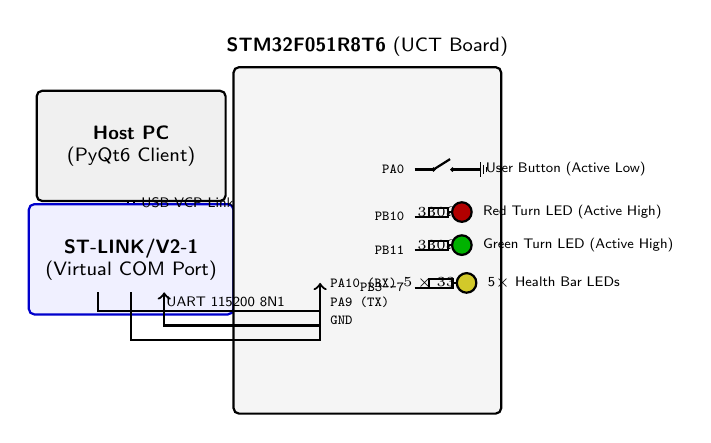
\begin{tikzpicture}[
    scale=0.60, every node/.style={font=\scriptsize\sffamily},
    chip/.style={draw=black, thick, fill=gray!8, rounded corners=2pt, minimum width=3.4cm, minimum height=4.4cm, align=center},
    pcbox/.style={draw=black, thick, fill=gray!12, rounded corners=2pt, minimum width=2.4cm, minimum height=1.4cm, align=center},
    pin/.style={font=\tiny\ttfamily},
    wire/.style={thick}
]
    % PC Block
    \node[pcbox] (pc) at (0, 2.4) {\textbf{Host PC}\\\scriptsize(PyQt6 Client)};

    % ST-LINK Block
    \node[draw=blue!80!black, thick, fill=blue!6, rounded corners=2pt, minimum width=2.6cm, minimum height=1.4cm, align=center] (stlink) at (0, 0) {\textbf{ST-LINK/V2-1}\\\scriptsize(Virtual COM Port)};

    % STM32F051 Block
    \node[chip] (stm) at (5.0, 0.4) {};
    \node[above] at (stm.north) {\textbf{STM32F051R8T6} (UCT Board)};

    % USB Connection
    \draw[wire, double, double distance=1.5pt] (pc) -- node[right, font=\tiny\sffamily] {USB VCP Link} (stlink);

    % UART Pins between ST-LINK and STM32
    \draw[wire, ->] (-0.7, -0.7) -- ++(0, -0.4) -| (4.0, -0.5) node[pin, right] {PA10 (RX)};
    \draw[wire, <-] (0.7, -0.7) -- ++(0, -0.7) -| (4.0, -0.9) node[pin, right] {PA9 (TX)};
    \draw[wire] (0, -0.7) -- ++(0, -1.0) -| (4.0, -1.3) node[pin, right] {GND};

    \node[font=\tiny\sffamily] at (2.0, -0.9) {UART 115200 8N1};

    % Peripherals on STM32
    % Reset Button
    \draw[wire] (6.0, 1.9) node[pin, left] {PA0} -- ++(0.4, 0) coordinate (b1);
    \draw[wire] (b1) ++(0.4, 0) coordinate (b2) -- ++(0.4, 0) coordinate (bgnd);
    \draw[wire] (b1) -- ++(0.35, 0.22);
    \filldraw (b1) circle (1pt) (b2) circle (1pt);
    \node[font=\tiny\sffamily, right] at (7.3, 1.9) {User Button (Active Low)};
    % Ground
    \draw[wire] (bgnd) -- ++(0.2, 0) coordinate (g1);
    \draw (g1) ++(0, 0.15) -- ++(0, -0.3);
    \draw (g1) ++(0.06, 0.10) -- ++(0, -0.2);
    \draw (g1) ++(0.12, 0.05) -- ++(0, -0.1);

    % Status LEDs
    \draw[wire] (6.0, 0.9) node[pin, left] {PB10} -- ++(0.3, 0) rectangle ++(0.4, 0.18);
    \node[font=\tiny] at (6.5, 1.0) {330$\Omega$};
    \draw[wire] (6.7, 1.0) -- ++(0.3, 0) node[circle, draw, fill=red!70!black, inner sep=2.5pt, label=right:\tiny Red Turn LED (Active High)] {};

    \draw[wire] (6.0, 0.2) node[pin, left] {PB11} -- ++(0.3, 0) rectangle ++(0.4, 0.18);
    \node[font=\tiny] at (6.5, 0.3) {330$\Omega$};
    \draw[wire] (6.7, 0.3) -- ++(0.3, 0) node[circle, draw, fill=green!70!black, inner sep=2.5pt, label=right:\tiny Green Turn LED (Active High)] {};

    % Health Bar LEDs
    \draw[wire] (6.0, -0.6) node[pin, left] {PB3--7} -- ++(0.3, 0) rectangle ++(0.5, 0.18);
    \node[font=\tiny] at (6.55, -0.5) {$5\times330\Omega$};
    \draw[wire] (6.8, -0.5) -- ++(0.3, 0) node[circle, draw, fill=yellow!80!black, inner sep=2.5pt, label=right:\tiny 5$\times$ Health Bar LEDs] {};
\end{tikzpicture}
\caption{System circuit diagram showing the physical UART interface routed through the on-board ST-LINK Virtual COM Port, the debounced user push-button on \texttt{PA0}, and GPIO status and health bar indicator LEDs.}
\label{fig:circuit}
\end{figure}

\subsection{Circuit Topology and Peripheral Integration}
Fig.~\ref{fig:circuit} illustrates the physical circuit topology connecting the STM32F051R8T6 microcontroller to the host PC and external user indicators:
\begin{itemize}
    \item \textbf{Host Serial Interface}: The microcontroller's \texttt{USART1} pins (\texttt{PA9} TX and \texttt{PA10} RX) route directly to the embedded ST-LINK/V2-1 interface on the Discovery board. The ST-LINK bridge enumerates as a USB Virtual COM Port (VCP) on the host machine, establishing bi-directional serial transfer at 115200 baud without requiring external USB-to-UART breakout boards or level shifters.
    \item \textbf{User Reset Button (\texttt{PA0})}: Connected to the momentary push-button. Configured in software as a floating input with an internal pull-up resistor (\texttt{GPIO\_PULLUP}). Pressing the button pulls \texttt{PA0} to ground. Software debouncing in \texttt{hardware.c} requires the input to remain stable low across a 50\,ms timing threshold before emitting \texttt{EVENT: RESET} and re-initializing game state.
    \item \textbf{Status and Turn Indicators (\texttt{PB10}, \texttt{PB11})}: Configured as active-high push-pull outputs driving visual indicator LEDs through current-limiting resistors. In \texttt{STATE\_IN\_PROGRESS}, \texttt{PB11} (Green) illuminates when Player~1 is active, while \texttt{PB10} (Red) illuminates during Player~2 or AI turns. In \texttt{STATE\_GAME\_OVER}, the winning player's LED blinks at a 250\,ms cadence.
    \item \textbf{Dynamic Health Bar (\texttt{PB3}--\texttt{PB7})}: A five-LED bar graph reflects the current number of surviving ships in the active player's fleet (or Player~1's health in AI mode). As ships are destroyed, corresponding LEDs are systematically extinguished, providing direct hardware feedback of combat progression.
\end{itemize}
